%\documentclass[t,handout]{beamer}
\documentclass{beamer}
\listfiles

\mode<presentation>
{
  \usetheme[deutsch,titlepage0]{KIT}
% \usetheme[usefoot]{KIT}
% \usetheme{KIT}

%%  \usefonttheme{structurebold}\inputencoding{latin1}

  \setbeamercovered{transparent}

  %\setbeamertemplate{enumerate items}[circle]
  \setbeamertemplate{enumerate items}[ball]

}

\newcommand*{\JOKE}{}%

%\date{10.05.2010}
%\DateText

\newlength{\Ku}
\setlength{\Ku}{1.43375pt}

\usepackage[utf8]{inputenc}
\usepackage[TS1,T1]{fontenc}
\usepackage{array}
\usepackage{multicol}
\usepackage{listings}
\usepackage{amsmath}
\usepackage{alltt}
\usepackage{graphicx}
\usepackage{tabularx}
\usepackage{hyperref}
\hypersetup{
	pdftitle={PSE: Blockchain-basiertes E-Voting - Implementierung -Präsentation},%
	,%
}

\lstset{language=Java,
	basicstyle=\verysmall,
	keywordstyle=\color{blue}\ttfamily,
	stringstyle=\color{red}\ttfamily,
	commentstyle=\color{green}\ttfamily,
	morecomment=[l][\color{magenta}]{\#},
	breaklines=true,
	breakatwhitespace=true,
	tabsize=2
}
%\usenavigationsymbols
%\usenavigationsymbols[sfHhdb]
%\usenavigationsymbols[sfhHb]

\title[]{PSE: Blockchain-basiertes E-Voting - Implementierung}
\subtitle{Präsentation}

\author{Tim Fröhlich, Achim Kriso, Philipp Schaback, David Schuldes, Artem Vasilev\\ Phasenverantwortlicher: Philipp Schaback}

\AuthorTitleSep{\relax}

\institute[]{KARLSRUHER INSTITUT FÜR TECHNOLOGIE (KIT)}

\TitleImage[width=\titleimagewd]{pictures/logo}

\newlength{\tmplen}

\newcommand{\verysmall}{\fontsize{6pt}{8.6pt}\selectfont}

\begin{document}

\begin{frame}

\maketitle

\end{frame}

\begin{frame}
\frametitle{Ein paar Zahlen:}
\begin{itemize}[<+->]
	\item \textbf{144} Sourcedateien
	\item \textbf{2801} Kommentarzeilen
	\item \textbf{6263} Codezeilen
\end{itemize}
\end{frame}

\ifdefined\JOKE
\begin{frame}
	\frametitle{Bekannte Probleme}
		\begin{itemize}
			\item<2> Hyperledger $:)$
		\end{itemize}
\end{frame}	
\fi

\begin{frame}
	\frametitle{Bekannte Probleme}
	\only<1,4->{
		\begin{itemize}
			\item<1,4-> \textbf{Fehlkonfiguration des Netzwerks}
			\item<4-> Datenbereinigung der Eingabe
			\begin{itemize}
				\item Sonderzeichen, Leerzeichen, etc.
			\end{itemize}
			\item<5-> GUI-Freeze bei Kommunikation mit der Blockchain	
			\item<6-> Diverse kleiner Bugs (siehe GitHub Issues)
		\end{itemize}
		\begin{block}<7>{}
			=> Lösung in der Qualitätssicherung
		\end{block}
	}
	\only<2>{
		\framesubtitle{Fehlkonfiguration des Netzwerks}
		\begin{figure}
			\vspace{-5pt}
			\centering
			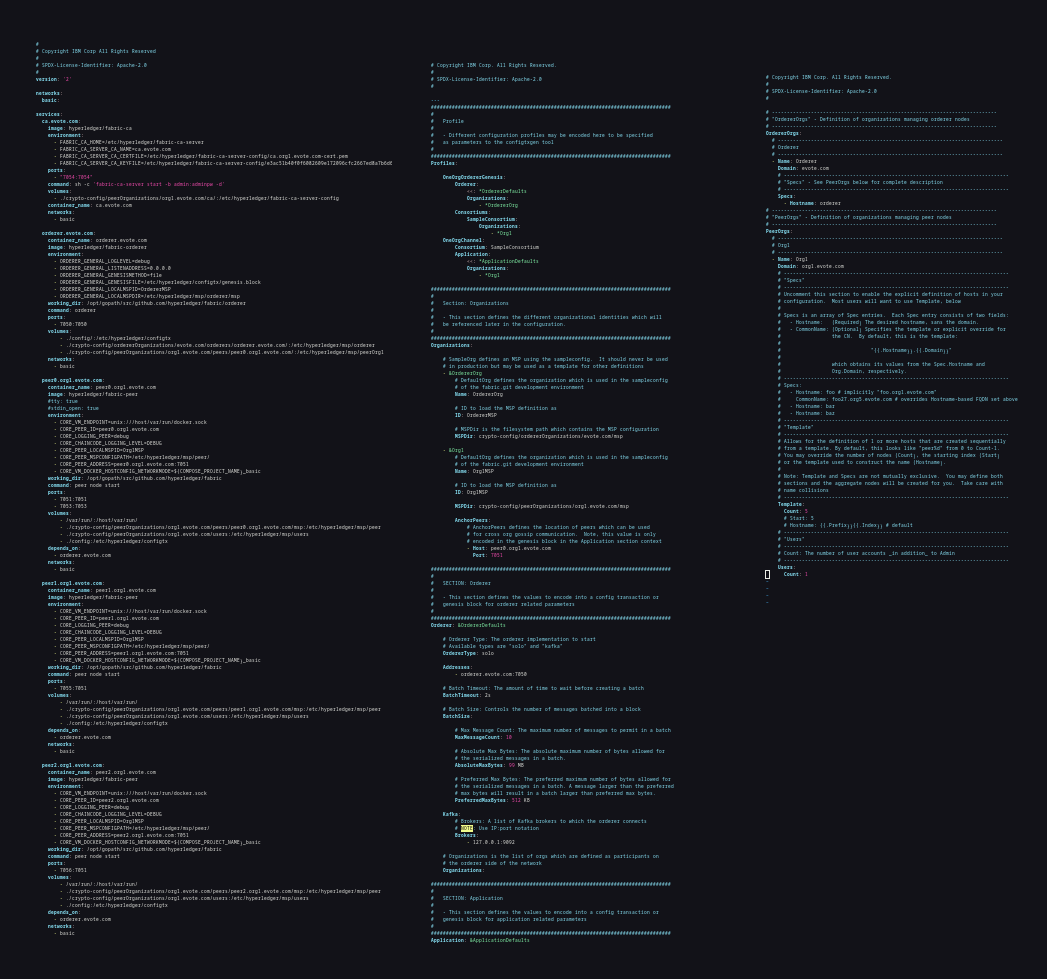
\includegraphics[width=\textheight]{pictures/collage}
		\end{figure}
	}
	\only<3>{
		\framesubtitle{Fehlkonfiguration des Netzwerks: Wolkengedöns™}
		\begin{figure}
			\vspace{-5pt}
			\centering
			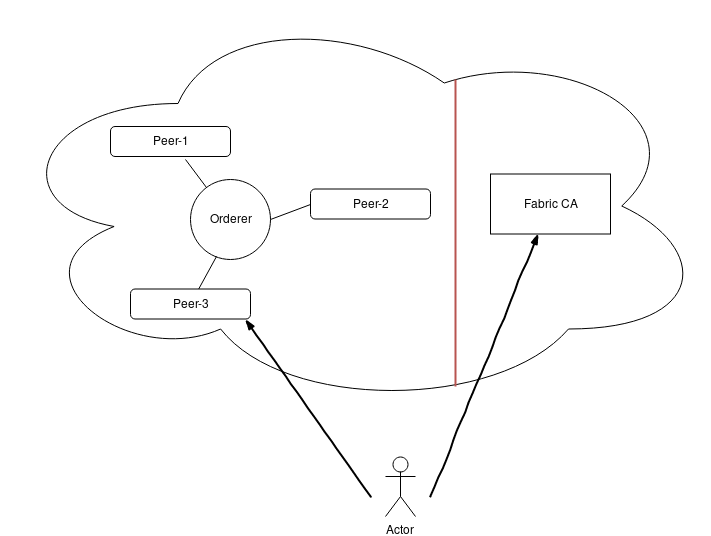
\includegraphics[width=\textheight]{pictures/wolkendiagramm}
		\end{figure}
	}
\end{frame}

\begin{frame}
\begin{center}
	\huge Demonstration
	\begin{figure}[h!]
		
\includegraphics[width=0.5\textwidth]{pictures/logo}
	\end{figure}
\end{center}
\end{frame}
\end{document}